\section{ХОД РАБОТЫ}

\subsection{Программа определения элемента списка по номеру}

Задание: разработать программу, определяющую элемент списка по его номеру.
Номер задается как аргумент.

Исходный код разработанной программы представлен на
рисунке~\ref{lst:el_by_idx}.

\lstinputlisting[style=source_code,numbers=left,numberstyle=\texttt,xleftmargin=2em,
                 caption=Исходный код программы,
                 language=prolog,label=lst:el_by_idx]{code/el_by_idx.pro}

Пример работы программы представлен на рисунке~\ref{fig:el_by_idx}.

\begin{figure}[h!]
  \centering
  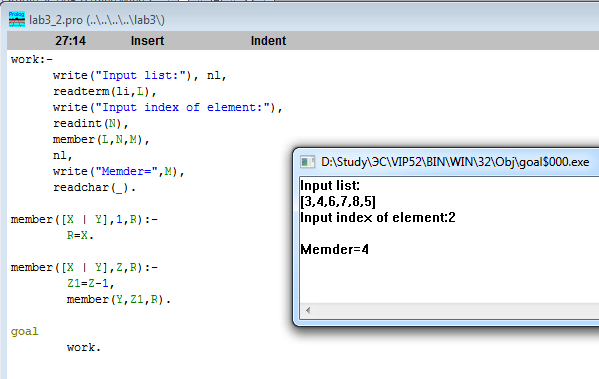
\includegraphics[width=92mm]{img/el_by_idx}
  \caption{Результат работы программы}
  \label{fig:el_by_idx}
\end{figure}


\subsection{Программа определения номера элемента в списке}

Задание: разработать программу, выдающую номер заданного элемента в списке.

Исходный код разработанной программы представлен на
рисунке~\ref{lst:idx_by_el}.

\lstinputlisting[style=source_code,numbers=left,numberstyle=\texttt,xleftmargin=2em,
                 caption=Исходный код программы,
                 language=prolog,label=lst:idx_by_el]{code/idx_by_el.pro}

Пример работы программы представлен на рисунке~\ref{fig:idx_by_el}.

\begin{figure}[h!]
  \centering
  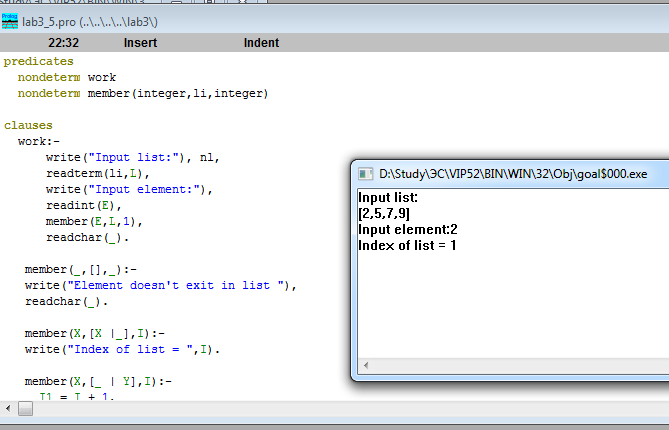
\includegraphics[width=92mm]{img/idx_by_el}
  \caption{Результат работы программы}
  \label{fig:idx_by_el}
\end{figure}


\subsection{Программа определения упорядоченности списка по \\ возрастанию}

Задание: разработать программу, определяющую,
упорядочен ли введенный список по возрастанию.

Исходный код разработанной программы представлен на
рисунке~\ref{lst:is_growing}.

\lstinputlisting[style=source_code,numbers=left,numberstyle=\texttt,xleftmargin=2em,
                 caption=Исходный код программы,
                 language=prolog,label=lst:is_growing]{code/is_growing.pro}

Пример работы программы представлен на рисунке~\ref{fig:is_growing}.

\begin{figure}[h!]
  \centering
  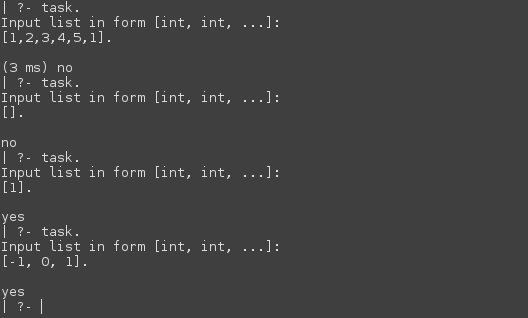
\includegraphics[width=120mm]{img/is_growing}
  \caption{Результат работы программы}
  \label{fig:is_growing}
\end{figure}


\subsection{TODO: Задача Паши}